\documentclass[10pt, a4paper, onecolumn]{scrartcl}
\usepackage{cite}  
\usepackage{times}
\usepackage{amsmath}
\usepackage{amsfonts}
\usepackage{amssymb}
\usepackage{graphicx}
\usepackage{listings}
\usepackage{enumitem} % used for list - no spaces between items
\usepackage[english]{babel} % English language/hyphenation
\usepackage[top=2cm, bottom= 3.2cm, left=2cm, right=2cm, columnsep=0.6cm]{geometry}
\usepackage{color} %red, green, blue, yellow, cyan, magenta, black, white
\definecolor{mygreen}{RGB}{28,172,0} % color values Red, Green, Blue
\definecolor{mylilas}{RGB}{170,55,241}
\usepackage{fancyhdr}
\pagestyle{fancyplain}
\fancyhead{}
\renewcommand{\headrulewidth}{0pt} % Remove header underlines
\fancyfoot[L]{} % Empty left footer
\fancyfoot[C]{} % Empty center footer
\fancyfoot[R]{\thepage} 
\usepackage{tikz}
\usetikzlibrary{shapes.geometric,arrows}
\usepackage[hidelinks]{hyperref}

\usepackage{sectsty} % Allows customizing section commands
\sectionfont{\centering\large\textbf}
\subsectionfont{\flushleft\normalsize\normalfont\textbf}
\subsubsectionfont{\flushleft\normalsize\normalfont\textit}
%\allsectionsfont{\centering} % Make all sections centered

\usetikzlibrary{shapes,arrows}
\tikzstyle{decision} = [diamond, draw, fill=blue!20, 
text width=4.5em, text badly centered, node distance=3cm, inner sep=0pt]
\tikzstyle{block} = [rectangle, draw, fill=blue!20, 
text width=5em, text centered, rounded corners, minimum height=4em]
\tikzstyle{line} = [draw, -latex']
\tikzstyle{cloud} = [draw, circle, fill=red!20, node distance=1.5cm,
minimum height=2em]
\tikzstyle{process} = [rectangle, minimum width=4cm, minimum height=2.5cm, text centered, draw=black, fill=green!20, node distance=6cm, text width = 2cm]
\setlength\parindent{0pt} % remove all indentations in document

%----------------------------------------------------------------------------------------
%	BEGIN DOCUMENT
%----------------------------------------------------------------------------------------
\newcommand{\horrule}[1]{\rule{\linewidth}{#1}}

\begin{document}
	
	\title{\normalfont \normalsize
		\textsc{University of Witwatersrand, Department of Electrical Engineering} \\ [10pt]
		\horrule{0.5pt} \\ [10pt]
		\huge Software Design Documentation \\
		\horrule{2pt} \\ [10pt]}
	\author{\textbf{\normalsize{Luka Cakic (671913), Ronen Freeman (386910), Devin Taylor (603956) and Matthew Marsden (609293)}} \\ [10pt]}
	\date {\normalsize \today}
	
	\maketitle
	
	\section{Introduction}
	
		The purpose of this documentation is to provide a detailed understanding of the structure of the software application. The documentation is primarily aimed at the software development team. The document aims to provide the software development team with a sense of guidance, thus ensuring the deliverables are in line with what is expected. \\
		
		The scope of the project, from a technical aspect, is that the design is composed of a front-end (client interface) and a back-end (server interface). The front end will consist of an interactive web application while the back-end will be a relational database. The database that will be used is PostgreSQL, primarily due to its compatibility with the chosen scripting language, \texttt{PHP5}. The functionality offered to the customer includes:
		
		\begin{itemize}
			\item Creating a user account
			\item Logging in to the application with the above created credentials
			\item Creating a shopping list
			\item Adding to and removing from an existing shopping list
			\item Creating multiple shopping lists with the above mentioned functionality
			\item Selecting their preferred means of route optimisation: fastest, shortest or cheapest
			\item Generating a route based on the shopping list and desired means of optimisation
		\end{itemize}
		
		The product is targeted at the general public. The reason being that all members of society are assumed to shop in some capacity. As a result of this the User Interface (UI) is required to be as simplistic as possible as this will avoid excluding those members of society that are not necessary technologically advanced. The primary purpose of the application being introduced is to better the overall well-being and state of mind of the general member of society. \\
		
		In order to configure the workstation to be compatible with the designed system framework it is necessary to follow the installation instructions provided in the products README or Installation and Initialisation documentation.
		
	\section{Design Considerations}
	
		\subsection{Assumptions and Dependencies}
		
			The success of the design relies heavily on the integration of the system with the Google Maps API. The API was selected as it is the most commercially trusted maps platform and it provides easy wrapper and integration functions for developers. Due to time constraints JavaScript wrapper functions were used as they were easier to implement, ideally these should be written in \texttt{PHP5} in order to ensure system wide integrity and compatibility. \\
			
			The application is designed to run through an Apache2 server, this is primarily due to the server being easy to configure. The Apache2 server is also known to integrate well with database management systems, which is essential for the functionality of the application. As previously mentioned the database management system that was chosen is PostgreSQL and the database interfacing language is \texttt{PHP5}. \\
			
			As the application back-end is designed upon Apache, the application hosting is platform independent. Due to it being a web application, and the front-end primarily being written is base HTML, the user interface is also browser independent. \\
			
			Due to the documented design being a simple prototype the design is subject to numerous changes. Firstly, as mentioned above, all interfacing languages should all be transported to \texttt{PHP5}. Secondly, it would be desired to be able to export the route to a mobile Google Maps application thus allowing the user to navigate the route without having to print it in advance. Thirdly, as the system currently calculates all possible permutations of routes and checks each one to determine the characteristics of the route, ultimately designing a `smart' system would be more ideal. The system will be capable of inferring which routes will most likely be the fastest thus reducing the number of routes that need to be checked. As a result the system will be able to provide a route in a much shorter time, as this aspect is currently the bottle-neck of the design. 
			
		\subsection{General Constraints}
		
			The primary constraint of the system is the acquisition of accurate and up-to-date data from the independent shops represented. The application is data driven thus a lack of data, or incorrect data, will directly hinder the functionality of the system. It is thus essential to be able to establish a system for continuously obtaining data from these shops. In conjunction with this it will also be necessary to set up a solid framework for interpreting the data, thus ensuring there will be no delays associated with this aspect.
		
		\subsection{Success Criteria}
		
			Due to the target market being broad, it is desired that the system be as simplistic in nature as possible. The more simplistic the UI, the more simplistic the server aspects can be. These concepts are what will allow the system to perform efficiently yielding maximum User Experience (UX). It can be noted that the greater the UX the greater the number of people that will utilise the application, which is ultimately the goal of the product. \\
			
		\subsection{Development Methods}
		
			The system is to be developed according to the SCRUM principles. This is ideally because an agile method of development is often preferred when designing an application. This is due to the frequent changes that the application is subject to. It is recommended that the reader familiarises themselves with the composed SCRUM selection document in order to understand the motivation behind the choices made.
	
	\section{Architectural Strategies}
	
		The primary architectural strategy implemented was that of the Model-View-Controller (MVC) design pattern, this design pattern is evident in the above discussions. The primary motivation for the implementation of this design pattern was due to the fact that the SCRUM design approach was implemented. Due to SCRUM, and the incremental development associated with it, the UI is subject to changes as a result of client feedback. The MVC pattern implemented is depicted below in Figure~\ref{mvc}.
		
		\begin{figure}[h]
				\centering
				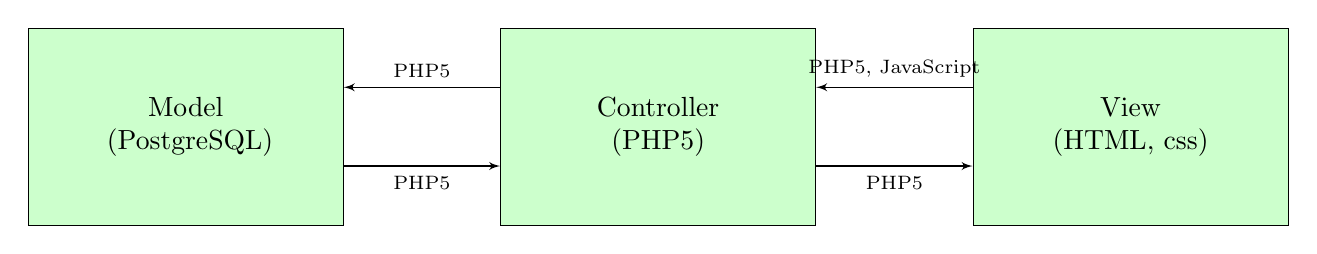
\begin{tikzpicture}[node distance = 2.1cm, auto]
				% Place nodes
				\node [process] (model) {Model \\ (PostgreSQL)};
				\node [process, right of=model] (cont) {Controller \\ (PHP5)};
				\node [process, right of=cont] (view) {View \\ (HTML, css)};
				% Draw edges
				\path [line] ([yshift=0.5cm]cont.west) -- node [anchor=south] {\scriptsize{PHP5}} ([yshift=0.5cm]model.east);
				\path [line] ([yshift=-0.5cm]model.east) -- node [anchor=north] {\scriptsize{PHP5}} ([yshift=-0.5cm]cont.west);
				\path [line] ([yshift=0.5cm]view.west) -- node [anchor=south] {\scriptsize{PHP5, JavaScript}} ([yshift=0.5cm]cont.east);
				\path [line] ([yshift=-0.5cm]cont.east) -- node [anchor=north] {\scriptsize{PHP5}} ([yshift=-0.5cm]view.west);
				\end{tikzpicture}
				\caption{MVC Design Pattern}
				\label{mvc}
		\end{figure}
	
		Certain additional strategies were implemented in order to reduce the amount of time taken to deliver a prototype system. These strategies are listed below. \\
		
		\begin{itemize}
			\item Database: As previously described the PostgreSQL was selected as the desired database structure primarily due to its compatibility with \texttt{PHP5}, a scripting language that the development team was familiar with.  
			\item JavaScript: The use of JavaScript to interface with the Google Maps API was primarily due to the fact that the code had previously been written and thus could simply be reused. This was acknowledged as a future aspect to be ported to \texttt{PHP5}, as previously mentioned.
			\item CSS: Majority of the \texttt{css} files implemented are due to previous experience with the open source packages. Due to the familiarity of how to interact with the packages it reduced the time required to obtain the desired appearance and behaviour of the UI.
		\end{itemize}
		
		Error handling is a fundamental aspect of the architectural design. The error handling was made the responsibility of the back-end. This was primarily to achieve and maintain the level of abstraction present in the design. The back-end is responsible for determining the required response to the user request (in error) and inform the front-end of the appropriate information to display. Certain errors that were accounted for are listed below:
		
		\begin{itemize}
			\item Incorrect credentials entered when creating an account
			\item Incorrect credentials entered when logging in to an existing account
			\item Item not found on the database when adding to the shopping list
			\item Item not found in the existing list when attempting to remove an item
			\item Unable to connect to the Google Maps API
		\end{itemize}

	\section{System Architecture and Data Design}
	
		The software behind the Shopping Route Recommender is designed in a responsibility-driven structure \cite{responsibility}. The responsibility-driven structure is primarily centred around the client/server model and the roles that each entity plays in the communication of data objects. The main aspect of the structure is to abstract the details of how the server handles the clients request, from the client. Therefore, the design is structured in such a way that the client can only specify the intent of the requests and the back-end is configured in such a way to handle to specified request by encapsulating the means of how it responds to the clients request.\\
		
		The system was divided up into multiple structures, of which objects could be created, in order to achieve this level of abstraction. The objects that could be created are listen below:
		
		\begin{itemize}
			\item User/Client objects
			\item Shopping list objects
		\end{itemize}
		
		The system is relatively simple in the sense that only two types of objects can be created. Different users can be created, all of them being encapsulated into the category of employee, and each user will be able to create multiple shopping list objects.\\
		
		The user is able to request that they be allowed to create one of the above mentioned objects, the server is then responsible for checking the credibility of the request and bringing about the appropriate response. If the request is successful the server will create and store the corresponding object on the database and notify the client of the success. if the request is unsuccessful then the server will not create the object and the client will be notified of such. \\
		
		The client objects are restricted from interacting with one another to ensure the confidentiality of information, these are classified as having private responsibilities \cite{responsibility}. The individual client objects have ownership over their respective shopping list objects, therefore forming an object neighbourhood \cite{responsibility}. The client objects have the ability to interface with the database to edit their shopping list objects. The abstraction is obtained by the client entering a list of additions/deletions while the server determines the integrity of the request and carries out the required request if it is possible. The client is notified of these changes when the shopping list displayed to them is altered. Therefore, in the described situation the client plays the role of a controller while the shopping list plays the role of an information holder \cite{responsibility}. The shopping list could be seen to display controller roles in the sense that the map objects are reliant on them, but it is still the responsibility of the client to control the generation of the route. \\
		
		A further factor that plays a role in the system is that of the map objects. The map objects are temporary in the sense that they have a limited life-time from the generation of the route to the completion of the route. The map objects are owned by the individual client objects and can also be viewed as having no responsibilities in the system but rather forming an information holder role.

	
	\begin{thebibliography}{1}
		\bibitem{responsibility} Wirfs-Brock, R. \textit{A Brief Tour of Responsibility-Driven Design}. Wirfs-Brock Associates. Available: \url{http://www.wirfs-brock.com/PDFs/A_Brief-Tour-of-RDD.pdf}. Last Access: 9 April 2016.
	\end{thebibliography}	
	
	
\end{document}